\documentclass{article}
\usepackage{graphicx, amsmath, booktabs}
\usepackage{amssymb}
\usepackage{hyperref}
\usepackage{algorithm}
\usepackage{algpseudocode}


\usepackage[backend=biber,style=numeric, sorting=none]{biblatex}
\addbibresource{references.bib}

\graphicspath{{../experiments/figs}{../experiments/plots}}

\title{Rolling Cointegration Pairs Strategy: \\Theory and Empirical Analysis}
\author{Lukas Schaller}
\date{\today}

\begin{document}
\maketitle

\begin{abstract}
We investigate a rolling-OLS cointegration pairs strategy that enters $\beta$-neutral long-short positions whenever the standardized spread (z-score) between two assets exceeds a pre-defined band and exits when the spread reverts.
Daily data for ten major cryptocurrencies (2022-2025) and eleven economically linked ETF pairs (2018-2025) are screened and tested for cointegration. Back-testing is performed to determine the optimal parameters for entry and exit thresholds and rolling window size.
ETF pairs that deliver Sharpe ratios around 1.0 and competitive maximum draw-downs are identified. Cryptocurrencies fail to yield satisfactory results.
The strategy is robust to transaction costs. We conclude that rolling cointegration is a viable alpha source for fundamentally related ETFs, even though absolute returns are modest.
\end{abstract}
\newpage
\tableofcontents
\setlength{\parskip}{0pt}
\clearpage  

\section{Theoretical Framework}
\label{sec:theory}

\subsection{Cointegration and the Pricing Spread}

Let \(P_t^{A}\) and \(P_t^{B}\) denote the prices of two assets $A$ and $B$ at time
\(t\).
A \emph{cointegrating relation} exists if there is a linear combination

\[
\varepsilon_t = P_t^{A} - (\alpha + \beta P_t^{B})
\]

such that \(\varepsilon_t\) is stationary.
In practice we estimate the coefficients \((\alpha,\beta)\) with ordinary least squares (OLS) from the model:

\[
P_t^{A} = \alpha + \beta P_t^{B} + \varepsilon_t.
\]
Here no assumptions are made about the distribution of the error term \(\varepsilon_t\).

\subsection{Decision Strategy}
We will assume that the pricing spread \(\varepsilon_t\) is a stationary process meaning that its mean and variance are constant over time.
Hence, we expect it to revert to its mean \(\mu\) over time when it deviates from it.
The strategy is to enter the market as soon as a gap between the price $P_t^{A}$ and the linear combination of the price $P_t^{B}$ exceeds a certain threshold.
We will go long on the asset that is underpriced and short the overpriced asset. As soon as the spread reverts to its mean, we close the position and take the profit. These ideas are extensively studied in the context of pairs trading \parencite{Vidyamurthy2004PairsTrading, Gatev2006PairsTrading}.

\emph{So, how to identify the entry and exit points?} 
We will use the z-score \(z_t\) of the residuals \(\varepsilon_t\) to determine the entry and exit points.
Recall that the z-score is defined as
\[
z_t = \frac{\varepsilon_t - \mu}{\sigma},
\]
where \(\mu\) is the mean and \(\sigma\) is the standard deviation of the residuals \(\varepsilon_t\).
Our strategy $S_0$ will then be
\begin{align}
    S_0 = \begin{cases}
        \text{Long A, Short B} &\;\;\text{if}\;\; z_t \le -z_{\mathrm{entry}},\\
        \text{Long B, Short A} &\;\;\text{if}\;\; z_t \ge +z_{\mathrm{entry}},\\
        \text{Exit} &\;\;\text{if}\;\; |z_t| < z_{\mathrm{exit}}.
    \end{cases} \label{eq:strategy_S0}
\end{align}
Here \(z_{\mathrm{entry}}\) and \(z_{\mathrm{exit}}\) are the defined entry and exit thresholds, respectively.

\subsection{Rolling Estimation}
Because in reality there is no guarantee that the cointegration relation holds forever, we cannot be sure that the residuals $\varepsilon_t$ are stationary for very long periods of time.
Hence, we will estimate the residuals as well as the corresponding z-score in a rolling window of length $w$:
\begin{align*}
(\alpha_t,\beta_t) &= \text{OLS}\left(P_{t-(w-1)}^{A},\dots,P_{t}^{A}\;
\text{; } P_{t-(w-1)}^{B},\dots,P_{t}^{B}\right), \\
\varepsilon_t &= P_t^{A} - (\alpha_t + \beta_t P_t^{B}), \qquad z_t = \frac{\varepsilon_t - \mu_{t}}{\sigma_{t}}, \\
\mu_{t} &= \text{mean} \left(\varepsilon_{t-(w-1)},\dots,\varepsilon_{t}\right), \qquad
\sigma_{t} = \text{stdev}\left(\varepsilon_{t-(w-1)},\dots,\varepsilon_{t}\right).
\end{align*}
This allows us to adapt to changing long-term trends in the prices of the considered assets.

\subsection{Further Mechanisms}
Recall the strategy $S_0$ defined in \eqref{eq:strategy_S0}. We can add an additional stop-loss mechanism to it, which will close the position if the current loss exceeds a certain threshold.
Another mechanism is to add an absolute threshold $\varepsilon_{\mathrm{min}}$ to the residuals, which needs to be exceeded before entering a position.
This can be very useful for low-volatility regimes, where the z-score even after small movements might be large due to a very small standard deviation.

\subsection{Testing for Stationarity}\label{sec:testing_for_stationarity}
To test whether the residuals \(\varepsilon_t\) are stationary, one can use the Augmented Dickey-Fuller (ADF) test \parencite{DickeyFuller1979}.
\paragraph{Augmented Dickey--Fuller test.}
For a series $x_t$ with mean 0 the ADF regression is
\[
\Delta x_t = \rho\,x_{t-1} + \sum_{i=1}^{p}\gamma_i\,\Delta x_{t-i} + u_t ,
\]
where $\Delta x_t = x_t - x_{t-1}$. $\rho$ and $\left(\gamma_i\right)_{i=1}^{p}$ are estimated coefficients and $u_t$ is a white noise error term.
We now test the null hypothesis $H_0:\,\rho = 0$ against the alternative $H_1:\,\rho < 0$.
The test statistic
\(
\tau = \hat{\rho}/\operatorname{SE}(\hat{\rho})
\)
is compared against MacKinnon critical values \parencite{MacKinnon2010CriticalValues}. The more negative the value of \(\tau\), the stronger the evidence against \(H_0\).
\newpage

\section{Data}
\paragraph{Data sources.}
\begin{itemize}
  \item \textbf{Exchange-Traded Funds (ETFs).}  Daily close prices were downloaded from \emph{Yahoo Finance} \parencite{yfinance} via the \texttt{yfinance} API in Python.
  \item \textbf{Cryptocurrencies.}  Daily prices were downloaded from \emph{Binance} \parencite{binance} using the \texttt{ccxt} Python library \parencite{ccxt}.
\end{itemize}
All series are sampled at a fixed \emph{1-day} interval.\footnote{Higher-frequency data approaches were not studied in this work.} For each asset we retain the most recent
1000 - 2000 trading days (roughly four to eight trading years), which is sufficient to calculate rolling 60-day estimates while leaving sufficient out-of-sample history for back-testing.
\paragraph{Data pre-processing.}
\begin{itemize}
    \item Prices of an asset pair are stored in a single \texttt{pandas DataFrame} \parencite{pandas} indexed by ISO date, ensuring data alignment.
    \item No currency conversion is required: both ETF and crypto prices are denominated in U.S. dollars.
\end{itemize}

\section{Screening results}
During the initial screening, 10 pairs of cryptocurrencies were tested. We calculated the $R^2$ of the OLS regression to filter out pairs in a first step. For the remaining pairs, we calculated the ADF test statistic to check for stationarity of the residuals. The results of the currency pairs with $R^2 \geq 0.7$ and $p_{\text{ADF}} < 0.05$ are summarized in Table 1. \footnote{The full set of cryptocurrencies of which all possible pairs were screened consists of BTC, ETH, XRP, LTC, BCH, ADA, DOT, LINK, XLM, and DOGE. All series are sampled from 01 Nov 2022 through 27 Jul 2025.}
\begin{table}[htbp]
\centering
\caption{Cryptocurrency pairs that passed the initial screening.}
\label{tab:crypto_screening}
    \begin{tabular}{lccc}
    \toprule
    Pair & $R^{2}$ & ADF statistic & $p_{\text{ADF}}$\\
    \midrule
    ETH/USDT - BCH/USDT  & 0.731 & $-3.58$ & 0.0061 \\
    ADA/USDT - XLM/USDT  & 0.793 & $-3.28$ & 0.0158 \\
    ADA/USDT - LINK/USDT & 0.722 & $-2.97$ & 0.0377 \\
    XRP/USDT - XLM/USDT  & 0.869 & $-2.89$ & 0.0468 \\
    \bottomrule
    \end{tabular}
\end{table}
Actual tests of the strategy performed even on these pairs yielded unsatisfactory results. The main reason seems to be that there is no strong enough force to push the spread back to its mean, because there is no economic reason for the prices to be cointegrated.
Hence, we decided to focus on pairs of ETFs. Here it is much more likely to find cointegrated pairs, because of economic relationships or just pairs of ETFs containing very similar assets. Results of the success of the strategy on ETF pairs can be found in section \ref{sec:empirical_results}.

\section{Back-Test Design}\label{sec:backtest}

\subsection{Parameter grid}
The back-test is run for different assets and parameter combinations.
\begin{itemize}
  \item \textbf{Entry threshold ($z_{\mathrm{entry}}$):} \{2.0, 2.5\}. This corresponds to a $> 97\%$ and $> 99\%$ confidence under normality assumptions.
  \item \textbf{Exit threshold ($z_{\mathrm{exit}}$):} \{0.05, 0.25\}.  Forces profit-taking once the spread has substantially decreased.
  \item \textbf{Rolling window ($w$):} \{40, 50, 60\} trading days for the
        OLS hedge ratio and z-score moments.
  \item \textbf{Absolute residual filter ($|\varepsilon_t|\ge\varepsilon_{\min}$):}
        \{0.0, 0.5\}.  Might be helpful in uncertain low-volatility regimes.
  \item \textbf{Stop-loss:} 5\,\% of invested capital per asset.
\end{itemize}
This yields $2^3 \cdot 3=24$ runs per asset pair.

\subsection{Position sizing and capital at risk}
All trades are $\beta$-neutral: one unit of asset $A$ is hedged by \(\beta_t \cdot P_t^A / P^B_t\) units of asset $B$.
The gross capital invested on day \(t\) is therefore
\[
G_t = \gamma \cdot \left( P_t^{A} + |\beta_t| P_t^{A} \right), \qquad \gamma \in \mathbb{R}_{>0},
\]
and \(\max_t G_t\) serves as capital-at-risk when computing total-return percentages. A 0.1\% transaction cost is applied to each entry action.

\subsection{Performance metrics}
For every run we record
\begin{itemize}
  \item total Sharpe ratio,
  \item Sharpe ratio during invested days,
  \item percentage of days invested,
  \item maximum draw-down,
  \item total return over capital-at-risk, and
  \item the same metrics for a 50-50 buy-and-hold benchmark.
\end{itemize}
\newpage

\section{Empirical results}\label{sec:empirical_results}

\subsection{Global grid sweep}
Table \ref{tab:top5_results} shows the top five parameter runs during back-testing on the parameter grid for different pairs of ETFs\footnote{The full set of ETF pairs screened consists of EEM / VWO, XLF / XLU, IWM / QQQ, XLK / XLY, TLT / IEF, EWJ / EZU, XLE / XLK, SHY / TLT, GDX / GLD, MTUM / SPLV, USO / IEF. All series are sampled from 01 Jan 2018 through 27 Jul 2025.}.
We observe that the best-performing pairs are TLT/IEF and EEM/VWO. TLT/IEF dominates in terms of Sharpe ratio, but is invested for a larger percentage of time and suffers from a larger maximum draw-down than EEM/VWO. The parameters chosen are similar, even though EEM/VWO seems to prefer a slightly higher entry threshold which also explains the difference in the percentage of days invested.
The detailed metrics of the best-performing run of TLT/IEF can be found in Table \ref{tab:metrics_best}.

\begin{table}[htbp]
\centering
\caption{Top five parameter runs sorted by total Sharpe ratio.}
\label{tab:top5_results}
\begin{tabular}{lrrrrrrrr}
\toprule
{Pair} &
{Sharpe} &
{Time in [\%]} &
{Max DD} &
$z_{\mathrm{entry}}$ &
$z_{\mathrm{exit}}$ &
$w$ &
$\varepsilon_{\min}$ \\
\midrule
TLT/IEF & 1.04 & 56.8 & $-4.33$ & 2.0 & 0.05 & 50 & 0.0 \\
TLT/IEF & 0.97 & 34.1 & $-3.57$ & 2.0 & 0.25 & 50 & 0.0 \\
TLT/IEF & 0.95 & 55.1 & $-4.33$ & 2.0 & 0.05 & 50 & 0.5 \\
EEM/VWO & 0.87 & 17.5 & $-0.38$ & 2.5 & 0.05 & 50 & 0.0 \\
EEM/VWO & 0.87 & 22.1 & $-0.50$ & 2.5 & 0.05 & 60 & 0.0 \\
\bottomrule
\end{tabular}
\end{table}

\begin{table}[htbp]
\centering
\caption{Key performance metrics for the first run of TLT/IEF from Table \ref{tab:top5_results}.}
\label{tab:metrics_best}
\begin{tabular}{l r}
\toprule
\textbf{Metric} & \textbf{Value} \\
\midrule
Sharpe ratio (total)            & 1.04 \\
Sharpe ratio (invested)         & 1.37 \\
Percentage of days invested     & 56.76\,\% \\
Maximum drawdown (strategy)     & --4.33\,\% \\
Total return (strategy)         & 5.52\,\% \\
Total return (50-50 benchmark)  & --4.62\,\% \\
Sharpe ratio (50-50 benchmark)  & 0.00 \\
Maximum drawdown (50-50 bench.) & --0.50\,\% \\
\bottomrule
\end{tabular}
\end{table}

Figure \ref{fig:heatmaps} shows the Sharpe ratio of the best-performing run for each pair of ETFs. The left panel varies the entry and exit thresholds, while the right panel varies the rolling window size and exit threshold.
One might recognize some of the best runs from the results in Table \ref{tab:top5_results} as some of cells in the heatmaps.

\begin{figure}[htbp]
\centering
\begin{minipage}{0.48\textwidth}
  \centering
  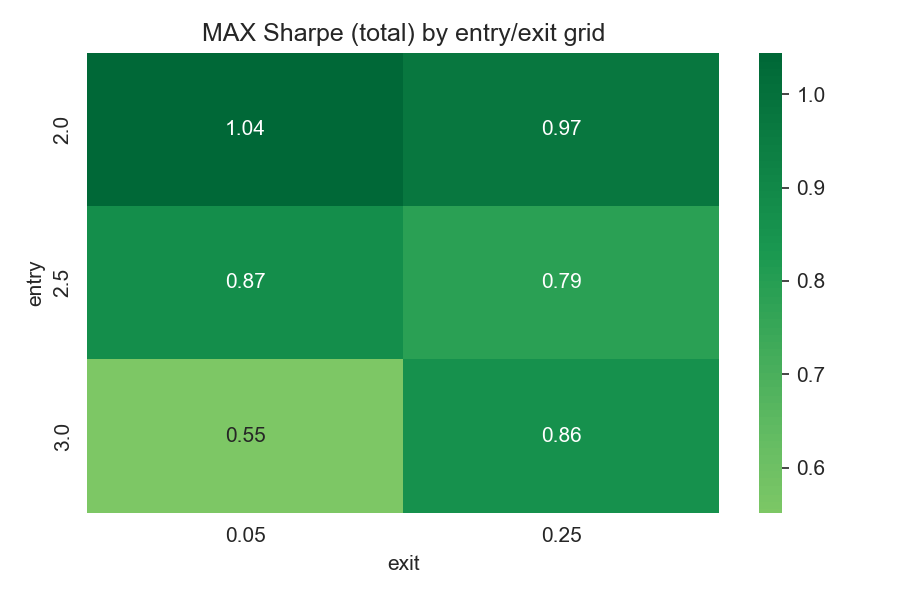
\includegraphics[width=\linewidth]{heat_entry_exit_max.png}
\end{minipage}\hfill
\begin{minipage}{0.48\textwidth}
  \centering
  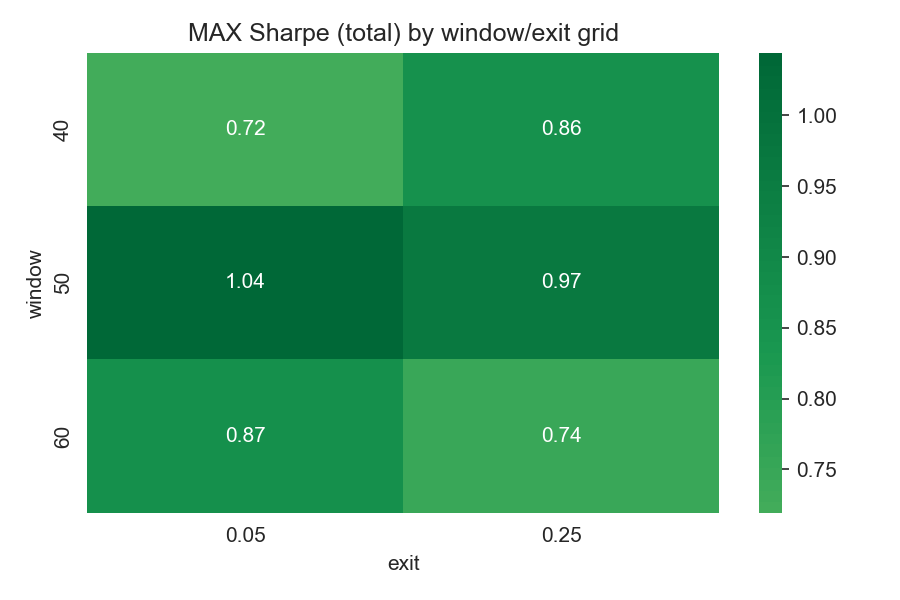
\includegraphics[width=\linewidth]{heat_window_exit_max.png}
\end{minipage}
\caption{Sharpe ratio of the best-performing run for each pair of ETFs. Left: entry vs.\ exit thresholds. Right: window size vs.\ exit threshold.}
\label{fig:heatmaps}
\end{figure}

\subsection{Case study: \texttt{TLT/IEF}}
We will now analyse the pair of ETFs \texttt{TLT} and \texttt{IEF}. \texttt{TLT} is the \textit{iShares 20+ Year Treasury Bond ETF} and \texttt{IEF} is the \textit{iShares 7-10 Year Treasury Bond ETF}. The back-test was run with a rolling window of $w=50$ days, an entry threshold of $z_{\mathrm{entry}}=2.0$, and an exit threshold of $z_{\mathrm{exit}}=0.05$. The absolute residual filter was set to $\varepsilon_{\min}=0$, and a stop-loss of 5\% was applied. The data ranges from 01 Jan 2018 to 27 Jul 2025 in 1 day intervals. \newline
Figure \ref{fig:trades_tlt_ief} shows the trades executed by the strategy. In the top panel the prices of the two ETFs are displayed and in the bottom panel z-score of the residuals is shown. The horizontal lines indicate the entry and exit thresholds. The strategy enters a position when the z-score crosses the entry threshold and exits when it crosses the exit threshold or the stop-loss is triggered.

\begin{figure}[htbp]
\centering
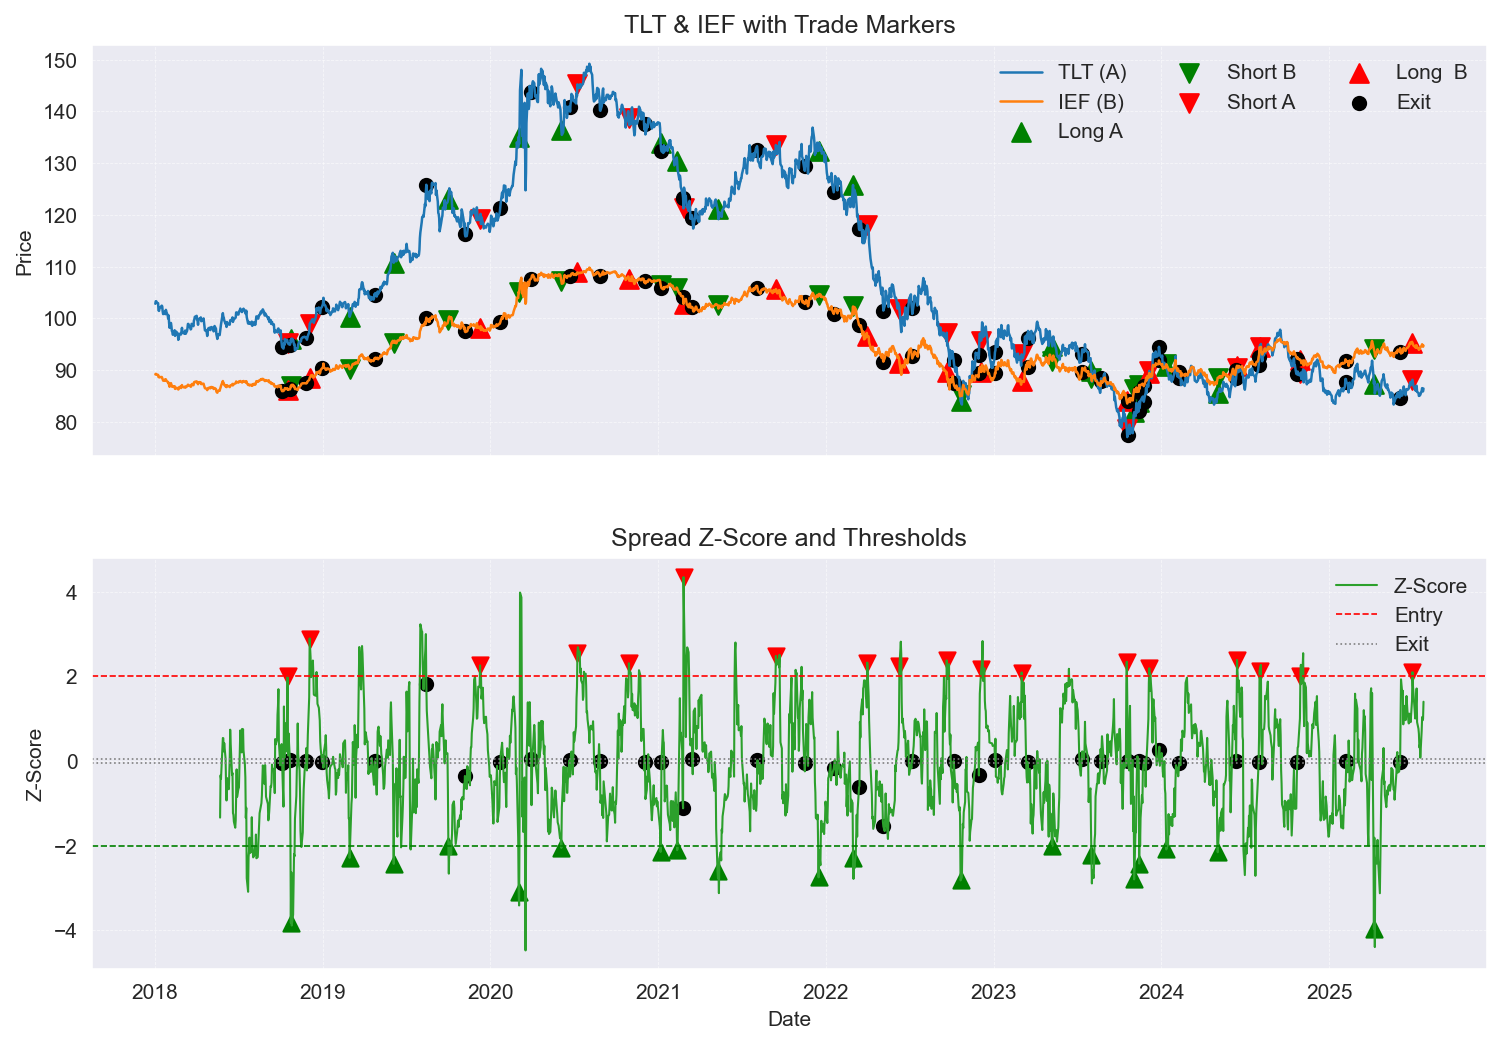
\includegraphics[width=\linewidth]{tlt_ief_trades.png}
\caption{Trades executed by the strategy on the pair of ETFs TLT/IEF. Top: prices of the two ETFs. Bottom: z-score of the residuals with entry and exit thresholds.}
\label{fig:trades_tlt_ief}
\end{figure}

\subsection{ADF as predictor of Sharpe ratio}
From the theory described in section \ref{sec:testing_for_stationarity} one could expect that the ADF test statistic is a good predictor of the Sharpe ratio of the strategy. Figure \ref{fig:adf_vs_sharpe} shows the ADF test statistic against the total Sharpe ratio for each pair of ETFs on their best set of parameters (by total Sharpe ratio).
But it is apparent that there is no reason to believe a more negative ADF statistic implies a higher Sharpe ratio. The correlation coefficient is approximately $0.544$ which would suggest a moderate positive relationship between the two variables. A similar picture emerges when looking at the Sharpe ratio during invested days or the difference of Sharpe ratio of the strategy and the 50-50 benchmark.
A reason for this could be that the ADF test statistic is not a good predictor of the stationarity of the residuals, but rather just a measure of how far the residuals are from being stationary.
\begin{figure}[htbp]
\centering
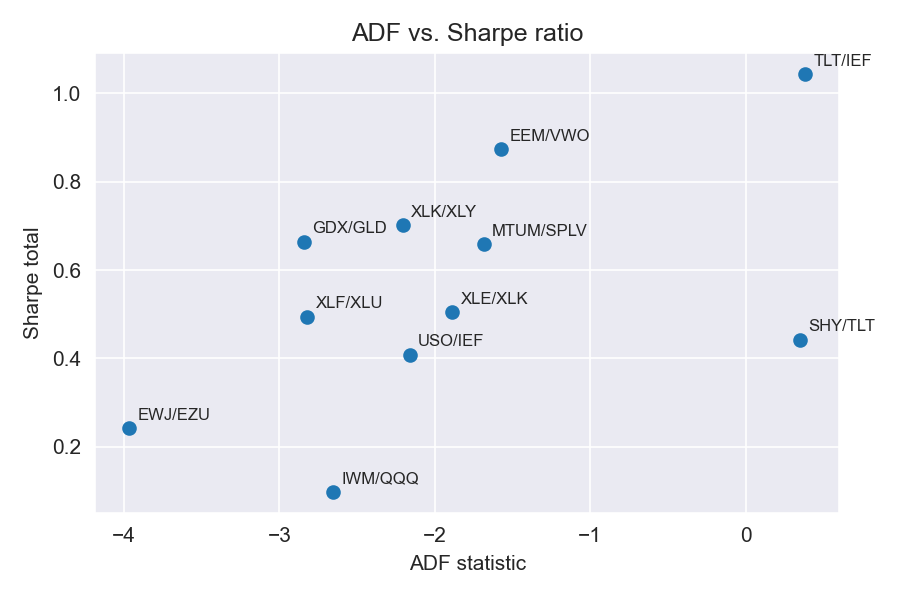
\includegraphics[width=0.8\linewidth]{adf_vs_sharpe_total.png}
\caption{ADF test statistic vs. total Sharpe ratio for each pair of ETFs on their best set of parameters.}
\label{fig:adf_vs_sharpe}
\end{figure}

\section{Conclusion}
We observed that the cointegration pairs trading strategy can be successfully applied to pairs of ETFs, yielding Sharpe ratios significantly larger than the naive 50-50 benchmark. Also, the maximum draw-down and the percentage of time invested could be reduced compared to the benchmark. The best performing parameters vary slightly between pairs, but a rolling window of 50 days, an entry threshold of 2.0, and an exit threshold of 0.05 seem to be a good choice. The ADF test statistic does not seem to be a good predictor of the strategy's Sharpe ratio.
In contrast to the ETFs, the strategy did not yield satisfactory results on pairs of cryptocurrencies, which is likely due to the lack of a strong economic relationship between their prices, as the most successful pairs of ETFs were very similar in their underlying assets.
Transaction costs were considered in the back-test. \newline
Even though the Sharpe ratios are significantly better than the naive benchmark, the absolute returns are modest given the long time span of several years. But a strength of this strategy is that profits can be made independent of overall market developments, based only on the relative developments of the given assets.\newline
Future work could focus on (i) exploring higher-frequency data, (ii) using more sophisticated entry and exit mechanisms as well as softer windowing, (iii) testing the strategy on other asset classes and (iv) investigating different tests for stationarity of the residuals as predictor for strategy success.
\newpage

\appendix
\section{Algorithm pseudo-code}
\begin{algorithm}[h!tbp]
\caption{Cointegration Pairs Trading Loop}
\label{alg:pairs}
\begin{algorithmic}[1]
\Require price series $(P^A_t, P^B_t)$, window $w$,
         thresholds $z_{\text{entry}}, z_{\text{exit}}$,
         stop-loss $s_{\text{SL}}$
\Statex
\For{$t = w, w+1, \dots, T$}
    \State \textbf{Estimate hedge ratio}
          \Comment{OLS on the last $w$ observations}
          \[
            (\alpha_t, \beta_t) \gets
            \operatorname{OLS}\bigl(P^{A}_{t-(w-1):t}
            \text{ on } P^{B}_{t-(w-1):t}\bigr)
          \]
    \State \textbf{Compute spread and z-score}
          \[
            \varepsilon_t = P^A_t - (\alpha_t + \beta_t P^B_t),\quad
            z_t = (\varepsilon_t - \mu_t)/\sigma_t
          \]
    \If{$\text{position}=0$}
        \If{$z_t < -z_{\text{entry}}$}
            \State long $A$, short $\beta_t B$
        \ElsIf{$z_t > z_{\text{entry}}$}
            \State short $A$, long $\beta_t B$
        \EndIf
    \Else
        \If{$|z_t| < z_{\text{exit}}$ \textbf{or} loss $> s_{\text{SL}}$}
            \State close position
        \EndIf
    \EndIf
    \State record PnL and update current position
\EndFor
\end{algorithmic}
\end{algorithm}

\newpage

\section{Additional figures}
\begin{figure}[htbp]
\centering
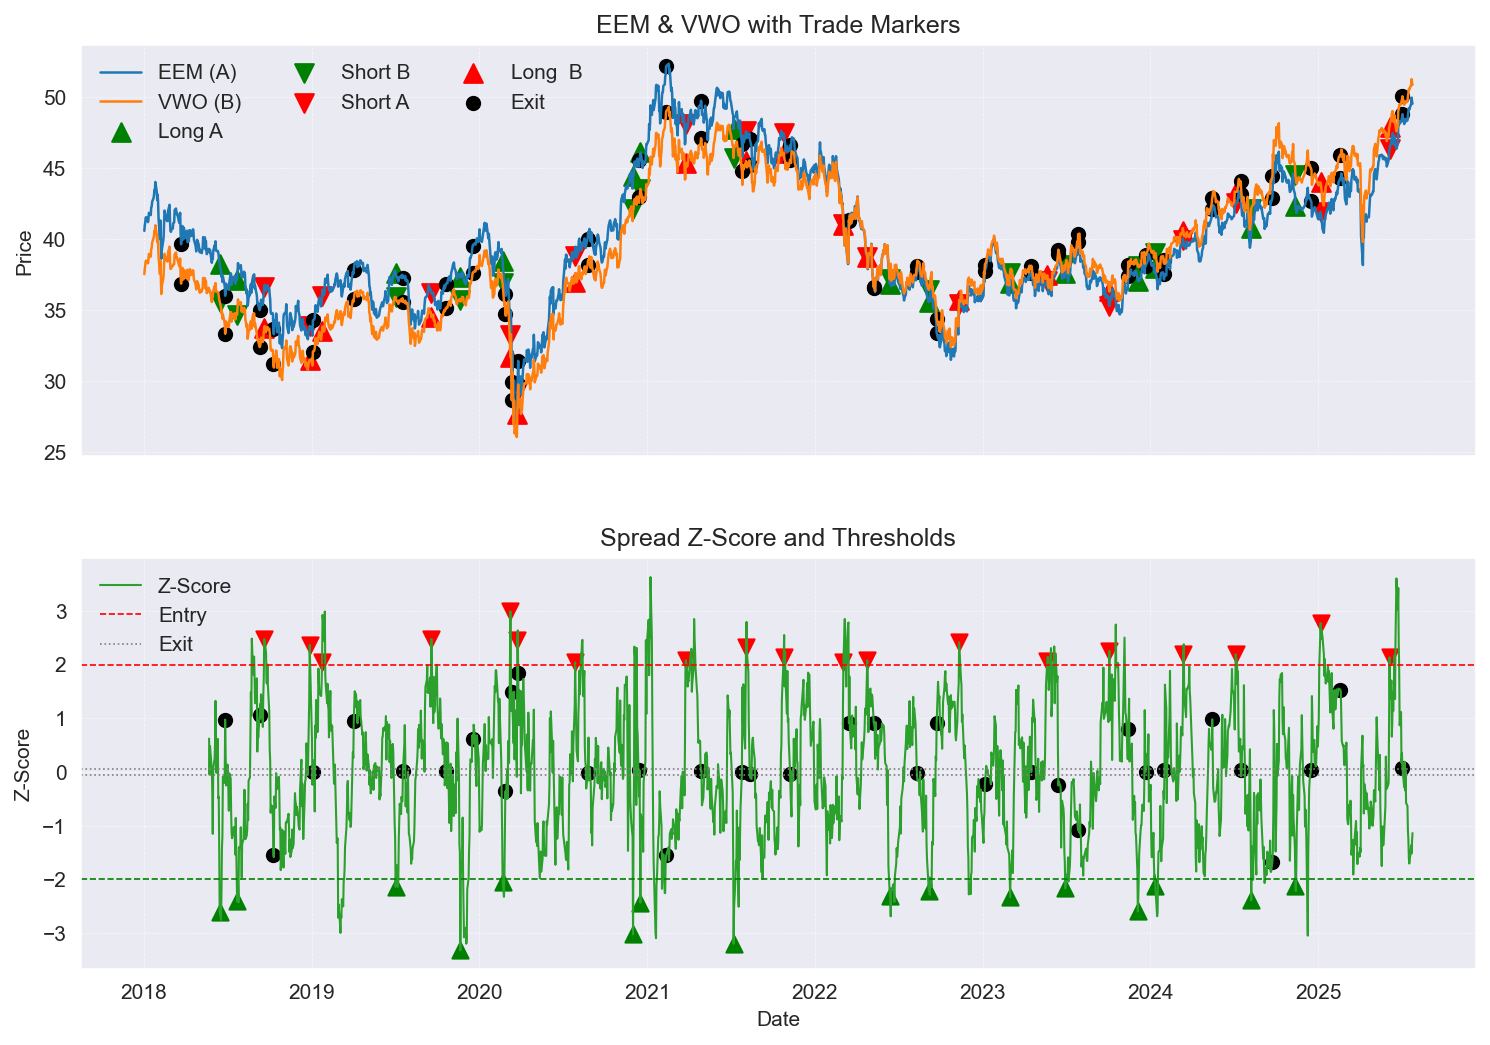
\includegraphics[width=\linewidth]{eem_vwo_trades.png}
\caption{Trades executed by the strategy on the pair of ETFs EEM/VWO. Top: prices of the two ETFs. Bottom: z-score of the residuals with entry and exit thresholds.}
\label{fig:trades_eem_vwo}
\end{figure}

\begin{figure}
\centering
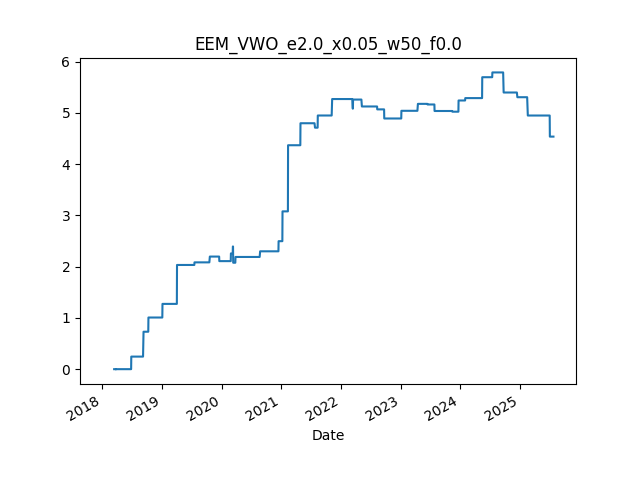
\includegraphics[width=0.8\linewidth]{EEM_VWO_e2.0_x0.05_w50_f0.0.png}
\caption{Absolute returns (USD) of the strategy on the pair of ETFs EEM/VWO with parameters $z_{\mathrm{entry}}=2.0$, $z_{\mathrm{exit}}=0.05$, $w=50$, and $\varepsilon_{\min}=0$. Capital-at-risk is 108 USD.}
\end{figure}

\begin{figure}
\centering
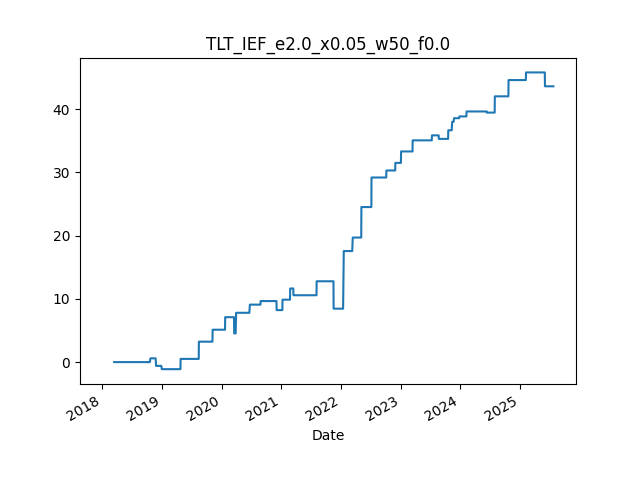
\includegraphics[width=0.8\linewidth]{TLT_IEF_e2.0_x0.05_w50_f0.0.png}
\caption{Absolute returns (USD) of the strategy on the pair of ETFs TLT/IEF with parameters $z_{\mathrm{entry}}=2.0$, $z_{\mathrm{exit}}=0.05$, $w=50$, and $\varepsilon_{\min}=0$. Capital-at-risk is 706 USD.}
\end{figure}

\clearpage
\printbibliography

\end{document}